\chapter{Fundamentals}
 \label{chap:funds}
 
 To understand the logic behind the implementations made in the thesis, we have to understand the execution workflow between the different modules (\emph{PyNESTML}, \emph{PyNEST} and \emph{NestKernel}). Those three modules may only be used together if we want to build our own custom neuron and synapse model, and therefore, in this chapter we will only focus on the execution of the simulation script using a user defined external model. \emph{PyNEST} does not enforce any order when to generate the code of the external model and install it, as along as the instance of the model is not used yet in the script. Thus, to keep everything simple and consistent, the simulation script will always start by generating all models and then installing them.
 
 
 
 
 
\section{PyNESTML The Code Generator}
 
 
The first step in each simulation script using an external model starts with calling the \texttt{generate\_target} function that is responsible mainly for everything in making the model available to the \emph{NestKernel} (generating the code, building the library and adding it to the installation path). The function takes different necessary parameters to ensure the correctness of the code generation. Mainly, the first parameter is the \texttt{input\_path} which holds the location of the model in the file system. This parameter can also be a list of paths, and in this thesis we only use the list when we want to co-generate the neuron and synapse models together and in all other cases we only generate one model at a time.
 


The second important parameter is the \texttt{codegen\_opts} which is responsible for providing extra information about the neuron  and if the code generation of the neuron should use a different logic in creating the library code. More importantly, this parameter is used for specifying the (\emph{neuron}, \emph{synapse}) pairs that are handled in \texttt{PyNESTML} to co-generate an efficient code and binding the \texttt{synapse} model only to the listed \texttt{neuron}. 

\emph{PyNESTML} can generate code for different target platforms, but for the scope of the thesis, we only focus on \emph{NEST} as the \texttt{target\_platform}. In the scope of the thesis, the remaining parameters are not of importance and do not affect the execution flow.

A \emph{neuron} model in \emph{NESTML} is the composition of different three blocks. The \emph{State} block defines a set of state variables representing the initial values of the model upon instantiation, and they can be updated during the simulation. The \emph{Parameter} block declares a set of variables depicting the model's constants that won't be modified during the simulation. Finally, we have the \emph{Internals} block. The block behaves like the \emph{Parameter} block, with the only difference that its variables can not be set outside the model (the user cannot explicitly modify the values before or after the simulation) and their initialization expression can only reference parameters or other internal variables.
 
 
The \emph{Neuron} model also has other important blocks, like the \emph{equation} block that handles \emph{differential equations} describing the time evolution of variables in the \emph{State} block. An \emph{update} block for updating the state of the neuron instance during the simulation run, and finally the \emph{input} and \emph{output} blocks for defining the incoming and outcoming signals respectively.

Each \emph{NESTML} neuron model is read by a parser and converted to an intermediate representation known as the abstract syntax tree (\texttt{AST}). After parsing the model and making sure that the described model is syntactically correct, the generated intermediate representation \texttt{AST} undergoes several transformations. Such transformations cover analyzing differential equations, processing the \emph{update} block and creating \emph{hooks} for the GNU Scientific Library. After applying these transformations, the \texttt{AST} goes through an optimization step, which includes \emph{constant folding} by eliminating expressions that calculate a value that can already be determined before code execution.
 
Figure \ref{fig:pynestml_workflow} below summarizes the complete workflow of the code generation in \emph{PyNESTML}. The process starts by feeding the \emph{.nestml} model to the code generator pipeline. A parsing and a validation steps take place, where the model is checked if it is syntactically correct and satisfies the code generator rules. Once the checks are complete, the pipeline moves to transforming the model into an intermediate representation in order to target different platforms. The third step is then the actual code generation, which is based on a set of templates written in \emph{Jinja} providing the implementation of the model in \texttt{C++} for the desired target platform. Finally, the last step in the pipeline controls the compilation and building of the model into \texttt{C++} \emph{shared library}  that can be loaded at runtime in the \emph{NestKernel}.


\begin{figure}[ht!]
\centering
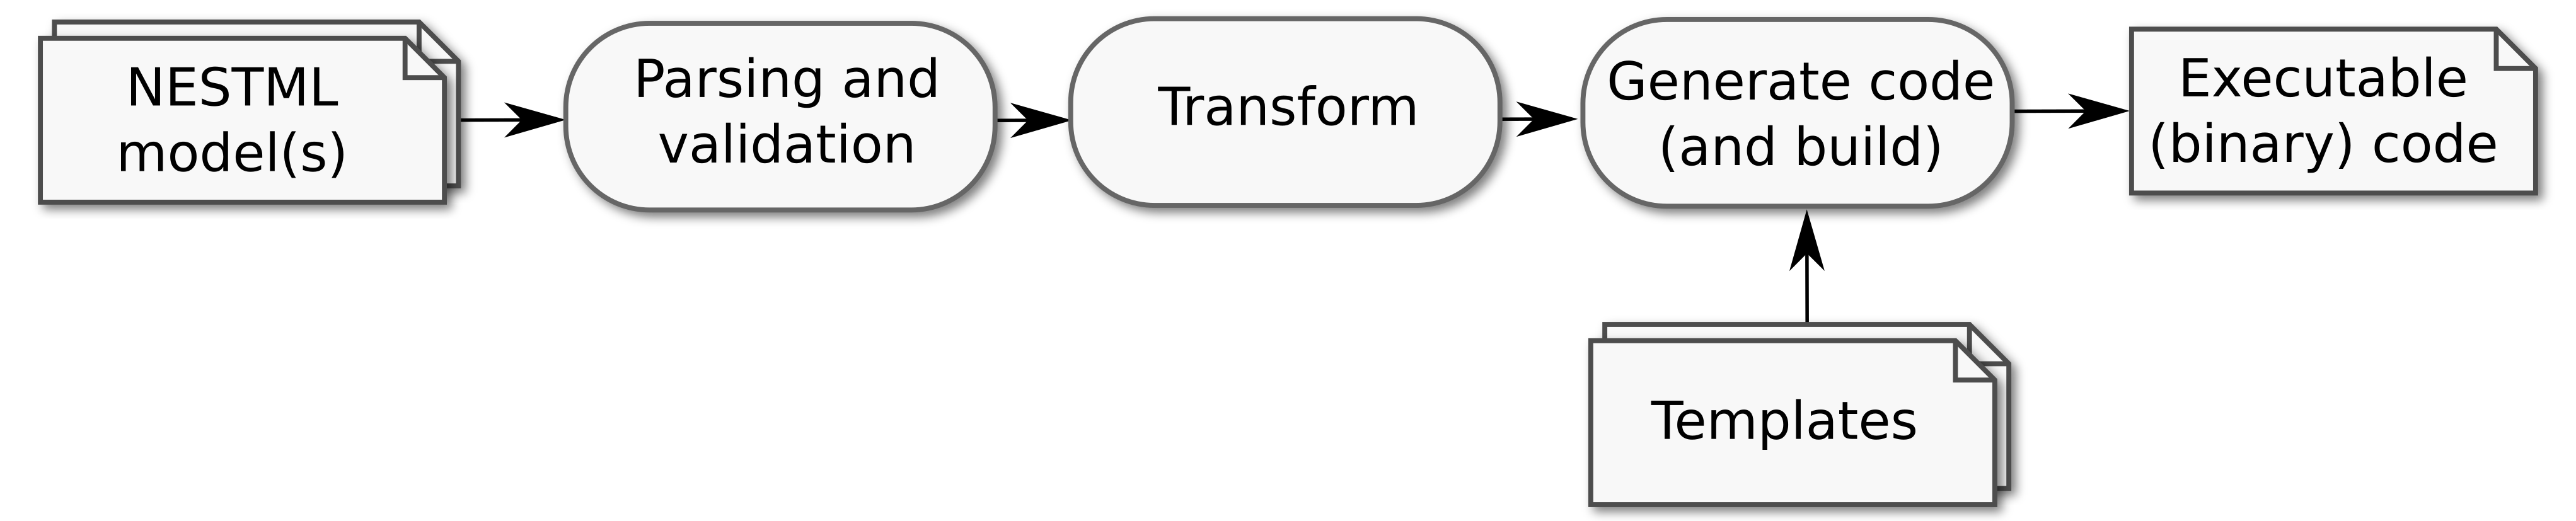
\includegraphics[width=0.8\textwidth]{src/pic/internal_workflow.png}
\caption{An overview of the processing workflow of \emph{PyNESTML}: The process starts by feeding the \emph{NESTML} models to the code generation pipeline. The first step in the pipeline starts by parsing the models and validating its syntax. Once the first step is completed, the models are transformed from a \emph{NESTML} files to an \emph{AST} objects. The pipeline moves to the next step by transforming the \emph{AST} objects. The transformation may extend the structure of the \emph{AST} by introducing new attributes or modify the name of the current model's attributes. Finally, we have the last step in the pipeline that takes the transformed \emph{AST} object and generates the \emph{C++} code for the model by using custom defined templates. Are all steps completed without any failure, the pipeline may compile and build the library of the generated code of the model on request and make it available for the simulation.}
%\source{\url{https://nestml.readthedocs.io/en/latest}}
\label{fig:pynestml_workflow}
\end{figure}



Is the model compiled, built and ready for use, the next step in the simulation is to make use of the model by introducing it to the \emph{NestKernel} and this happens by the call to \texttt{nest.Install()}. Therefore, in the subsequent section, we examine the execution path taken by registering new models in \emph{NEST}.

\section{NestKernel The Simulation Backend}


This section serves as a basic introduction to the most important functionalities that will be affected by the new implementation in \autoref{chap:vec}. Registering new custom models and creating new nodes are the first steps in each simulation script, and usually the user should not worry about how nodes are created. Once the model is registered, the \emph{NestKernel} creates a \emph{factory} object responsible for instantiating nodes from the model and managing any modification made to the model by the user during the simulation. To further understand the \emph{factory} concept in registering and creating nodes, we have to take a deeper look at the source code and inspect the important steps required for making the correct execution of the simulation. In the subsequent section, firstly we review the logic behind registering nodes and secondly, how to create node instances from these models.

From the start, we have mentioned that \emph{PyNEST} is the Python interface for executing the \emph{NestKernel} functions. That is actually not totally true. Each function call in \emph{PyNEST} is directly forwarded to the \emph{SLI} engine \citep{gewaltig2007nest}. \text{SLI} is a stack-based language derived from PostScript \citep{adobe1990postscript}, and it is outside the scope of the thesis.

Figure \ref{fig:layer} below depicts the three layers that are responsible for running the simulation, from the Python interface to the \texttt{C++} layer. \emph{PyNEST} takes the arguments from the simulation scripts and processes the arguments to make them ready for the \emph{SLI} interface functions. \texttt{SLI} then starts objects conversion and calls the exposed functions in the \emph{NestKernel}.

\begin{figure}[h!]
\centering
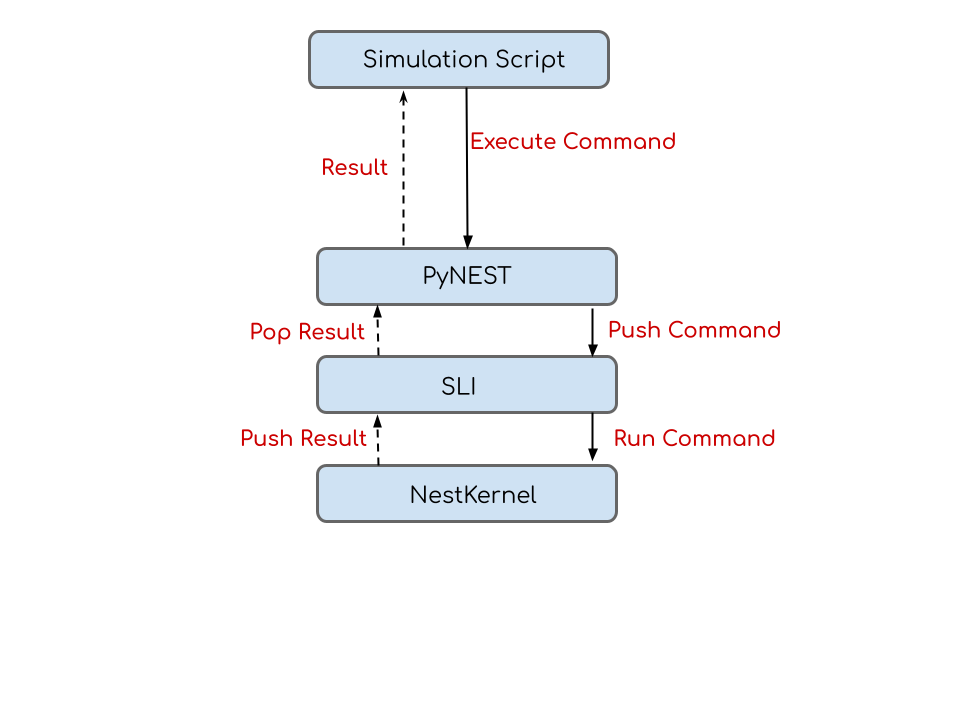
\includegraphics[width=0.8\textwidth]{src/pic/layers.png}
\caption{\emph{NEST} layers: At the top level, we have the user simulation script that imports the \emph{PyNEST} module. The \emph{PyNEST} functions represents an intermediate layer between the simulation script and the \emph{NestKernel}. They simply prepare the arguments of the command and push them onto the stack in \emph{SLI}. \emph{SLI} retrieves then the command and the arguments from the stack and call the corresponding function in the \emph{NestKernel}. The result then takes the opposite path, from the \emph{NestKernel} to the simulation script. After the completion of the command in the context of the \emph{NestKernel}, the results are pushed onto the stuck, and then \emph{SlI} comes again and removes them from the stack and make them available to the simulation script.}
\label{fig:layer}
\end{figure}

\subsection{Registering New Models}

For abstraction, we use \texttt{N} as the custom model class type that will be registered and show the workflow in the message sequence diagram depicted in the   \autoref{fig:nestknerl_register}.  Every custom model generated by \emph{PyNESTML} is shipped with two main components (see \autoref{fig:sli_install}). The first component is the implementation of the model in \texttt{C++} and the second component is the derived class from the \texttt{SLIModule}, and it is responsible for registering the model in the \emph{Nestkernel}. By calling the \texttt{nest.Install} function
with the model library name as parameter, \emph{SLI} searches for the library in the provided paths and dynamically loads it. Upon loading, \emph{SLI} calls the \texttt{init()} functions in the derived \texttt{SLIModule} class. The \texttt{SLIModule} instance calls the \texttt{register\_node\_model}  in the \texttt{ModelManager} class. The function required mainly two items. The first is the Class  type name of the model as in the \emph{template} name and secondly, the name of the model that will be available to the user to use. 

The \texttt{register\_node\_model} function checks if there exists another model under the same name and only proceed to registering the model if its name is unique. Afterwards, a new instance of the \texttt{GenericModel<T>} class is created with our model \texttt{N} as the substituted type (i.e., \texttt{T = N}). In fact, the \texttt{GenericModel} class works as a factory responsible for creating the instances of \texttt{N}, which means that  the user can not explicitly call the constructor of \texttt{N} and each creation of \texttt{N} is done by the \texttt{GenericModel}. Finally, the \texttt{ModelManager} takes control again, sets the model parameters (i.e., \texttt{ID}) and lastly creates a \texttt{proxy} objects of the model in each \emph{thread}. The \texttt{proxy} nodes are only required for nodes residing in remote processes, and they are meant for boosting the performance during connections setup and simulation. The \texttt{register\_node\_model} returns then the new \texttt{ID} of the model to \texttt{SLIModule} which itself returns the same \texttt{ID} to the initiator of the \texttt{install} command in \emph{SLI}.
 
 
 \begin{figure}[ht!]
\centering
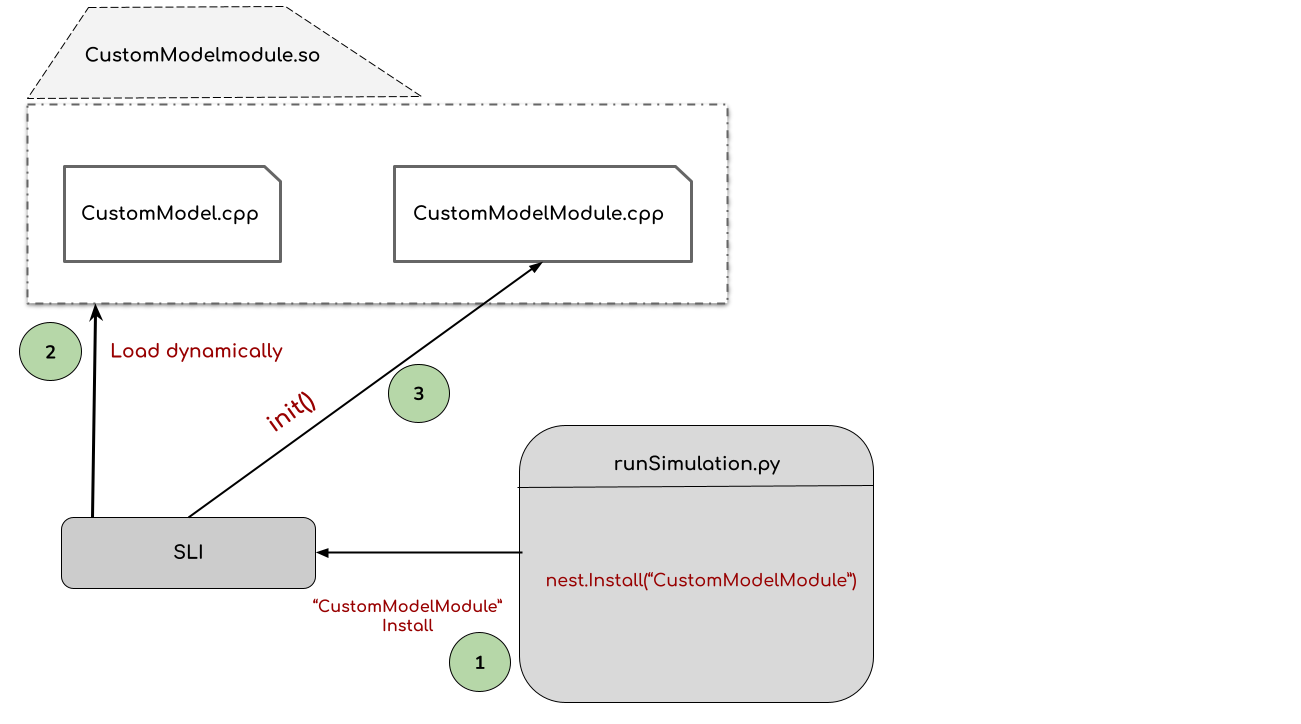
\includegraphics[width=1.2\textwidth,height=1.2\textheight,keepaspectratio]{src/pic/install_command.png}
\caption{Installing an external module: Each generated model comes with two main \emph{CPP} files. The first is implementing the model's logic and functionalities, and the second for registering the model in the \emph{NestKernel}. The process as always starts at the simulation script level, the call to \texttt{nest.Install} with the library name as the argument to the function starts the process of registering the model. The function pushes the command name and the library onto the stack that will be processed by the \emph{SLI} routine. \emph{SLI} loaded the library and creates an instance of the \texttt{SLIModule} representing the loaded module. The instance initiates then the call to the \texttt{init} function that starts the registering workflow of the new generated model in the \emph{NestKernel}.}
\label{fig:sli_install}
\end{figure}

\vspace{0.5cm}
\begin{figure}[ht!]
\centering
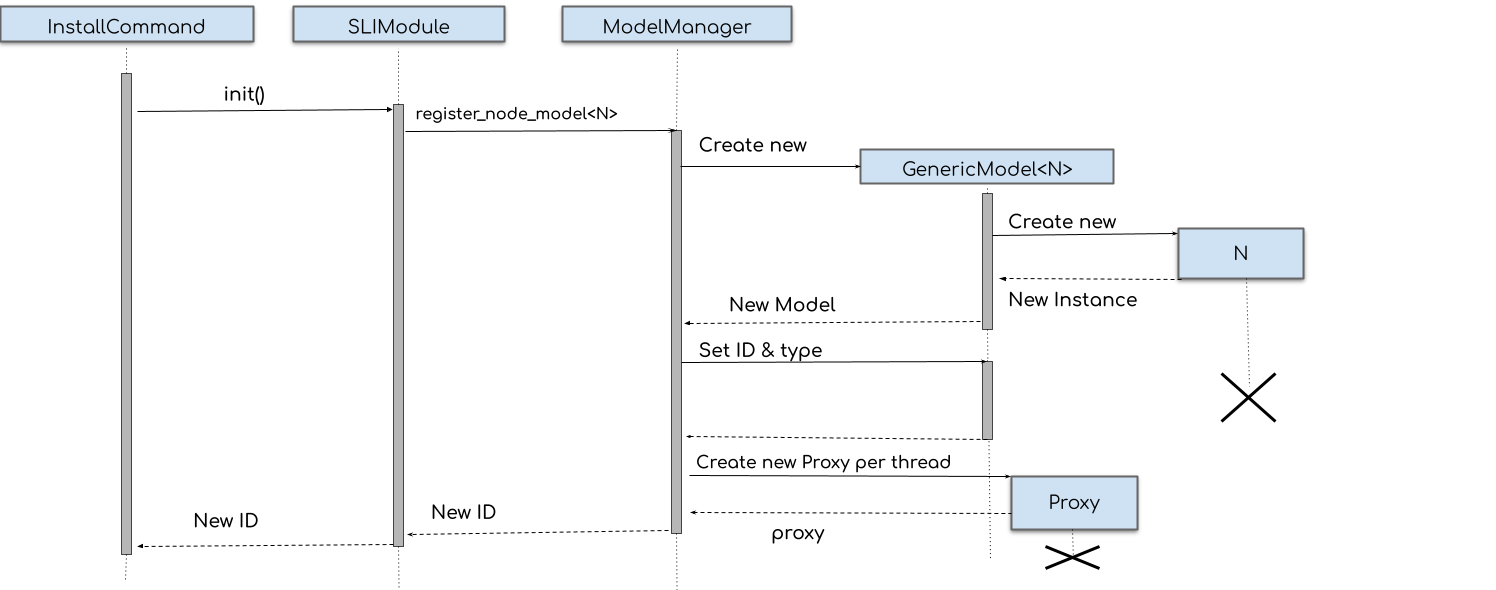
\includegraphics[width=1.2\textwidth,height=1.3\textheight,keepaspectratio]{src/pic/register.png}
\caption{ Registering new models in the \emph{NestKernel}: The message sequence chart depicts the interaction between the components in the \emph{NestKernel} responsible for registering new custom external models.}
\label{fig:nestknerl_register}
\end{figure}

\subsection{Creating New Nodes}

In this subsection, we focus on three components in the \emph{NestKernel}. The \texttt{NodeManager} which is responsible for creating nodes, handling the distribution of nodes over the available \emph{threads}.
It is important to keep in mind that each node is exactly assigned to one thread and each thread can only modify its nodes, non-local nodes are represented by \emph{proxies}. Also, each thread knows the total number of the created nodes. The second component
is the \texttt{GenericModel}, and as we have mentioned in the previous subsection that it plays the role of a \emph{factory} responsible for creating the real instances of the registered model. Finally, the registered model \texttt{N} which provides an implementation for \emph{cloning} that is required of creating new nodes.
Upon requesting the creation of $n$ nodes, the \texttt{NodeMananger} calls the \texttt{GenericModel} to create an instance of the registered model, which just creates a new empty copy of the model and returns it to the \texttt{NodeManager}. \autoref{fig:nestknerl_creation} depicts the steps involved in creating a new node.


\begin{figure}[ht!]
\centering
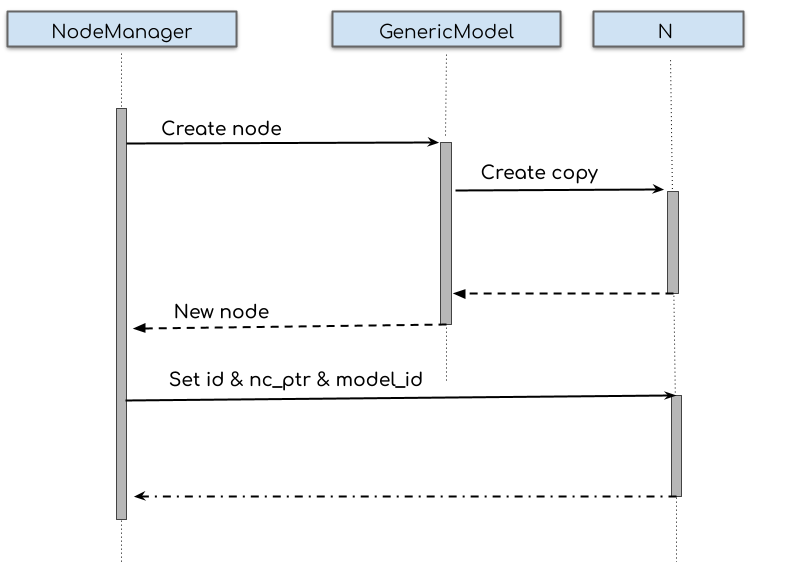
\includegraphics[width=1\textwidth,height=1\textheight,keepaspectratio]{src/pic/nodes_creation.png}
\caption{Creating new instances of the registered models in the \emph{NestKernel}: The message sequence chart depicts the interaction between the components in the \emph{NestKernel} responsible for creating new instances of any arbitrary registered model.}
\label{fig:nestknerl_creation}
\end{figure}


\section{PyNEST The Simulation Frontend}

\emph{PyNEST} and the \emph{NestKernel} are completely separated and independent modules. The only way for both of them to communicate is through the \texttt{SLI} interface. As shown in \autoref{fig:pynest} from \citep{epp}, \emph{PyNEST} is split into two layers. The \emph{low-level API} is responsible for ensuring the smooth communication between \emph{Python} and \emph{SLI} by providing the necessary functionalities for converting data from \emph{SLI} to \emph{Python} and vice versa. The \emph{low-level API} is based on the \emph{Python C API}. It uses mainly three functions to communicate with \emph{SLI}. The \texttt{sli\_push()} function for pushing the function's arguments of the \emph{SLI} command onto the stack, \texttt{sli\_pop} for retrieving the returned value of the command from the stack and finally the \texttt{sli\_run} for executing the command.  the \texttt{sli\_push} and \texttt{sli\_pop} are also responsible for converting the data (arguments and results) between both interfaces.



 The \emph{high-level API} provides the necessary functions for creating the network and running the simulation. Using the three provided functions in the \emph{low-level API} is not convenient and might not be very intuitive. Therefore, the \emph{high-level API} solves this problem by wrapping the \texttt{SLI} functions. It covers all the functionalities in \emph{SLI} by using the functions from the \emph{low-level API}, making all \emph{SLI} commands available.
 
 Each simulation script is based on the \emph{high-level API} functions. The \texttt{Create} function is responsible for creating new instances of the registered models. It takes four parameters, the model name, the number of instances, the new model parameters values and lastly a spatial distribution of the nodes. Only the model name is a required parameter, and the others are optional. Omitting the number of instances, the \texttt{Create} function returns one single instance. Discarding the model parameters values, the created node will have the default model values and finally, the nodes will not have any spatial distribution if the \texttt{spatial} parameter is omitted. The returned value of the function is a \texttt{NodeCollection} object. The \texttt{NodeCollection} class is a compact representation of the nodes in the \texttt{high-level API} interface. Apart from the \texttt{Create} function, all functions in \emph{PyNEST} expect a \texttt{NodeCollection} object in order to query or modify the created nodes. The \texttt{NodeCollection} stores only the \texttt{ids} of the nodes it contains, and thus less conversion overhead between \emph{SLI} and \emph{PyNEST}. 



An important feature of the \texttt{NodeCollection} class, that it only stores a contiguous set of nodes. Thus, creating many nodes only requires storing the position of the first and the last position of the nodes in the list. Thus, the \texttt{NodeCollection} always holds a list of contiguous blocks. Since the class is also \emph{iterable}, it supports indexing, splitting and concatenating.  


The \texttt{NodeCollection} allows also retrieve different values from the created nodes by calling the \texttt{get} functions. Depending on the number of provided keys, the \texttt{get} function returns either a \emph{list} or \emph{dictionary} containing the values of the given keys. We can also change the values by calling the \texttt{set} function. Setting is a bit complicated, as the given value might have different interpretation in the \emph{NestKernel}. Depending on the number of the nodes in the \texttt{NodeCollection} and the type of value (\emph{single} or \emph{list}), the setting might affect single nodes or all of them.

Another important feature is copying models. \emph{PyNEST} and \texttt{Nestkernel} allow users to copy existing models and assign them a new name and different \emph{default-initial} values. The function responsible for copying the models is called \texttt{CopyModel}.

Creating a network is made by calling the \texttt{Connect} function that takes two \texttt{NodeCollection} objects as the \emph{pre-synaptic (source)} and \emph{post-synaptic (target)} elements with extra parameters specifying the type of the connection and a set of rules defining the connection rules (i.e., controlling degree).

Finally, we have the \texttt{Simulate} function  with the time $t$ as parameter, which simulates the created network for $t$ milliseconds.

Of course the \emph{PyNEST} module has other important functions to provide, like inspecting the topology of the created network, changing the number of working threads and configuring the \emph{kernel} attributes, but we are mainly interested in the above-mentioned functions that will be used in designing and implementing the architecture for the \emph{JIT} module in the following chapter.
 
 

\begin{figure}[ht!]
\centering
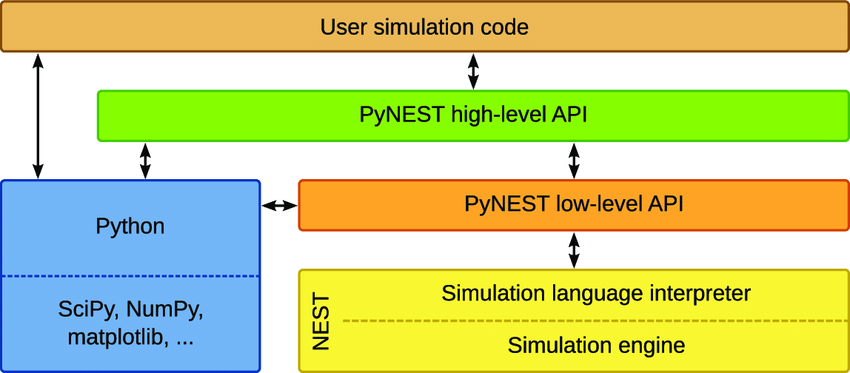
\includegraphics[width=1\textwidth,height=1\textheight,keepaspectratio]{src/pic/The-architecture-of-PyNEST-The-lowest-level-is-the-simulation-engine-It-is-used-by.png}
\caption{The architecture of \emph{PyNEST}: The figure is taken from \citep{epp}, and it shows the main communication levels between the user code and the \emph{NestKernel}. The lowest level is the simulation engine. It is used by
the simulation language interpreter and by the \emph{PyNEST} low-level API. The\emph{PyNEST} high-level
API uses the low-level API to communicate with the simulation engine. The user’s simulation
code can use functions from \emph{PyNEST}, from Python, and from its extension modules.}
\label{fig:pynest}
\end{figure}




